
\documentclass[11pt]{article}
\usepackage[margin=0.78in]{geometry}
\usepackage{booktabs}
\usepackage{longtable}
\usepackage{tabularx}
\usepackage{array}
\usepackage{graphicx}
\usepackage{float}
\usepackage{hyperref}
\usepackage{amsmath}
\hypersetup{colorlinks=true, linkcolor=blue, urlcolor=blue}
\setlength{\parskip}{0.45em}
\setlength{\parindent}{0pt}
\renewcommand{\arraystretch}{1.12}

\title{Strategy Exit-Policy Robustness\\\large LaTeX Source Report}
\author{ML-Based Trading of TP2-Inspired Violations in SPY American Call Options}
\date{June 22, 2026}

\begin{document}
\maketitle

\section{Purpose}

This report checks whether the four TP2 strategy denominations produce stable
conclusions across exit definitions. It uses the existing liquid-exit strategy
labels and does not recalculate raw TP2 detection.

\section{Exit Policies}

The policies are: reversion-day exit, first-liquid-on-or-after-reversion exit,
reversion plus 1/3/5 trading sessions, and selected-leg expiration payoff.

\section{Policy Strategy Summary}
\begin{tabular}{llrrrrrr}
\toprule
Exit & Strategy & Valid & Valid rate & Hit rate & Net P\&L & Median return & Mean hold \\
\midrule
Reversion day & T1 & 80,226 & 35.4\% & 37.8\% & -\$49.16M & -2.1\% & 2.58 \\
Reversion day & T2 & 100,685 & 44.4\% & 31.8\% & -\$3.26M & -3.1\% & 2.69 \\
Reversion day & K1 & 105,591 & 46.6\% & 25.9\% & -\$19.35M & -2.5\% & 2.62 \\
Reversion day & K2 & 79,965 & 35.3\% & 30.9\% & -\$24.58M & -1.8\% & 2.57 \\
Reversion +1 & T1 & 71,746 & 31.7\% & 56.1\% & -\$5.41M & 1.0\% & 3.83 \\
Reversion +1 & T2 & 98,279 & 43.4\% & 29.4\% & -\$25.67M & -3.9\% & 3.98 \\
Reversion +1 & K1 & 93,864 & 41.4\% & 28.3\% & -\$21.77M & -1.5\% & 3.93 \\
Reversion +1 & K2 & 71,366 & 31.5\% & 44.3\% & -\$2.15M & -0.8\% & 3.82 \\
Reversion +3 & T1 & 60,986 & 26.9\% & 52.4\% & -\$22.54M & 0.5\% & 6.51 \\
Reversion +3 & T2 & 91,832 & 40.5\% & 37.6\% & -\$4.17M & -2.5\% & 6.85 \\
Reversion +3 & K1 & 75,827 & 33.5\% & 29.1\% & -\$13.85M & -1.6\% & 6.66 \\
Reversion +3 & K2 & 60,789 & 26.8\% & 46.7\% & -\$7.38M & -0.5\% & 6.50 \\
Reversion +5 & T1 & 48,826 & 21.5\% & 61.4\% & -\$17.30M & 2.4\% & 9.55 \\
Reversion +5 & T2 & 83,312 & 36.8\% & 34.6\% & -\$27.25M & -3.5\% & 9.92 \\
Reversion +5 & K1 & 57,898 & 25.6\% & 33.9\% & -\$10.75M & -1.0\% & 9.65 \\
Reversion +5 & K2 & 48,488 & 21.4\% & 48.6\% & -\$10.64M & -0.2\% & 9.54 \\
First liquid & T1 & 83,846 & 37.0\% & 37.6\% & -\$49.09M & -2.3\% & 2.73 \\
First liquid & T2 & 101,337 & 44.7\% & 31.8\% & -\$3.34M & -3.1\% & 2.70 \\
First liquid & K1 & 106,232 & 46.9\% & 25.8\% & -\$19.40M & -2.5\% & 2.63 \\
First liquid & K2 & 83,703 & 36.9\% & 30.5\% & -\$24.42M & -1.9\% & 2.73 \\
Expiration & T1 & 188,077 & 83.0\% & 27.2\% & -\$32.16M & -17.5\% & 12.53 \\
Expiration & T2 & 215,929 & 95.3\% & 70.9\% & \$194.35M & 6.8\% & 28.59 \\
Expiration & K1 & 177,943 & 78.5\% & 68.8\% & -\$118.56M & 6.6\% & 26.42 \\
Expiration & K2 & 177,943 & 78.5\% & 28.0\% & \$173.84M & -17.9\% & 26.42 \\
\bottomrule
\end{tabular}

\section{Within-Policy Rankings}
\begin{tabular}{llrrrr}
\toprule
Exit & Strategy & P\&L rank & Return rank & Net P\&L & Median return \\
\midrule
Reversion day & T2 & 1 & 4 & -\$3.26M & -3.1\% \\
Reversion day & K1 & 2 & 3 & -\$19.35M & -2.5\% \\
Reversion day & K2 & 3 & 1 & -\$24.58M & -1.8\% \\
Reversion day & T1 & 4 & 2 & -\$49.16M & -2.1\% \\
First liquid & T2 & 1 & 4 & -\$3.34M & -3.1\% \\
First liquid & K1 & 2 & 3 & -\$19.40M & -2.5\% \\
First liquid & K2 & 3 & 1 & -\$24.42M & -1.9\% \\
First liquid & T1 & 4 & 2 & -\$49.09M & -2.3\% \\
Reversion +1 & K2 & 1 & 2 & -\$2.15M & -0.8\% \\
Reversion +1 & T1 & 2 & 1 & -\$5.41M & 1.0\% \\
Reversion +1 & K1 & 3 & 3 & -\$21.77M & -1.5\% \\
Reversion +1 & T2 & 4 & 4 & -\$25.67M & -3.9\% \\
Reversion +3 & T2 & 1 & 4 & -\$4.17M & -2.5\% \\
Reversion +3 & K2 & 2 & 2 & -\$7.38M & -0.5\% \\
Reversion +3 & K1 & 3 & 3 & -\$13.85M & -1.6\% \\
Reversion +3 & T1 & 4 & 1 & -\$22.54M & 0.5\% \\
Reversion +5 & K2 & 1 & 2 & -\$10.64M & -0.2\% \\
Reversion +5 & K1 & 2 & 3 & -\$10.75M & -1.0\% \\
Reversion +5 & T1 & 3 & 1 & -\$17.30M & 2.4\% \\
Reversion +5 & T2 & 4 & 4 & -\$27.25M & -3.5\% \\
Expiration & T2 & 1 & 1 & \$194.35M & 6.8\% \\
Expiration & K2 & 2 & 4 & \$173.84M & -17.9\% \\
Expiration & T1 & 3 & 3 & -\$32.16M & -17.5\% \\
Expiration & K1 & 4 & 2 & -\$118.56M & 6.6\% \\
\bottomrule
\end{tabular}
\begin{figure}[H]
  \centering
  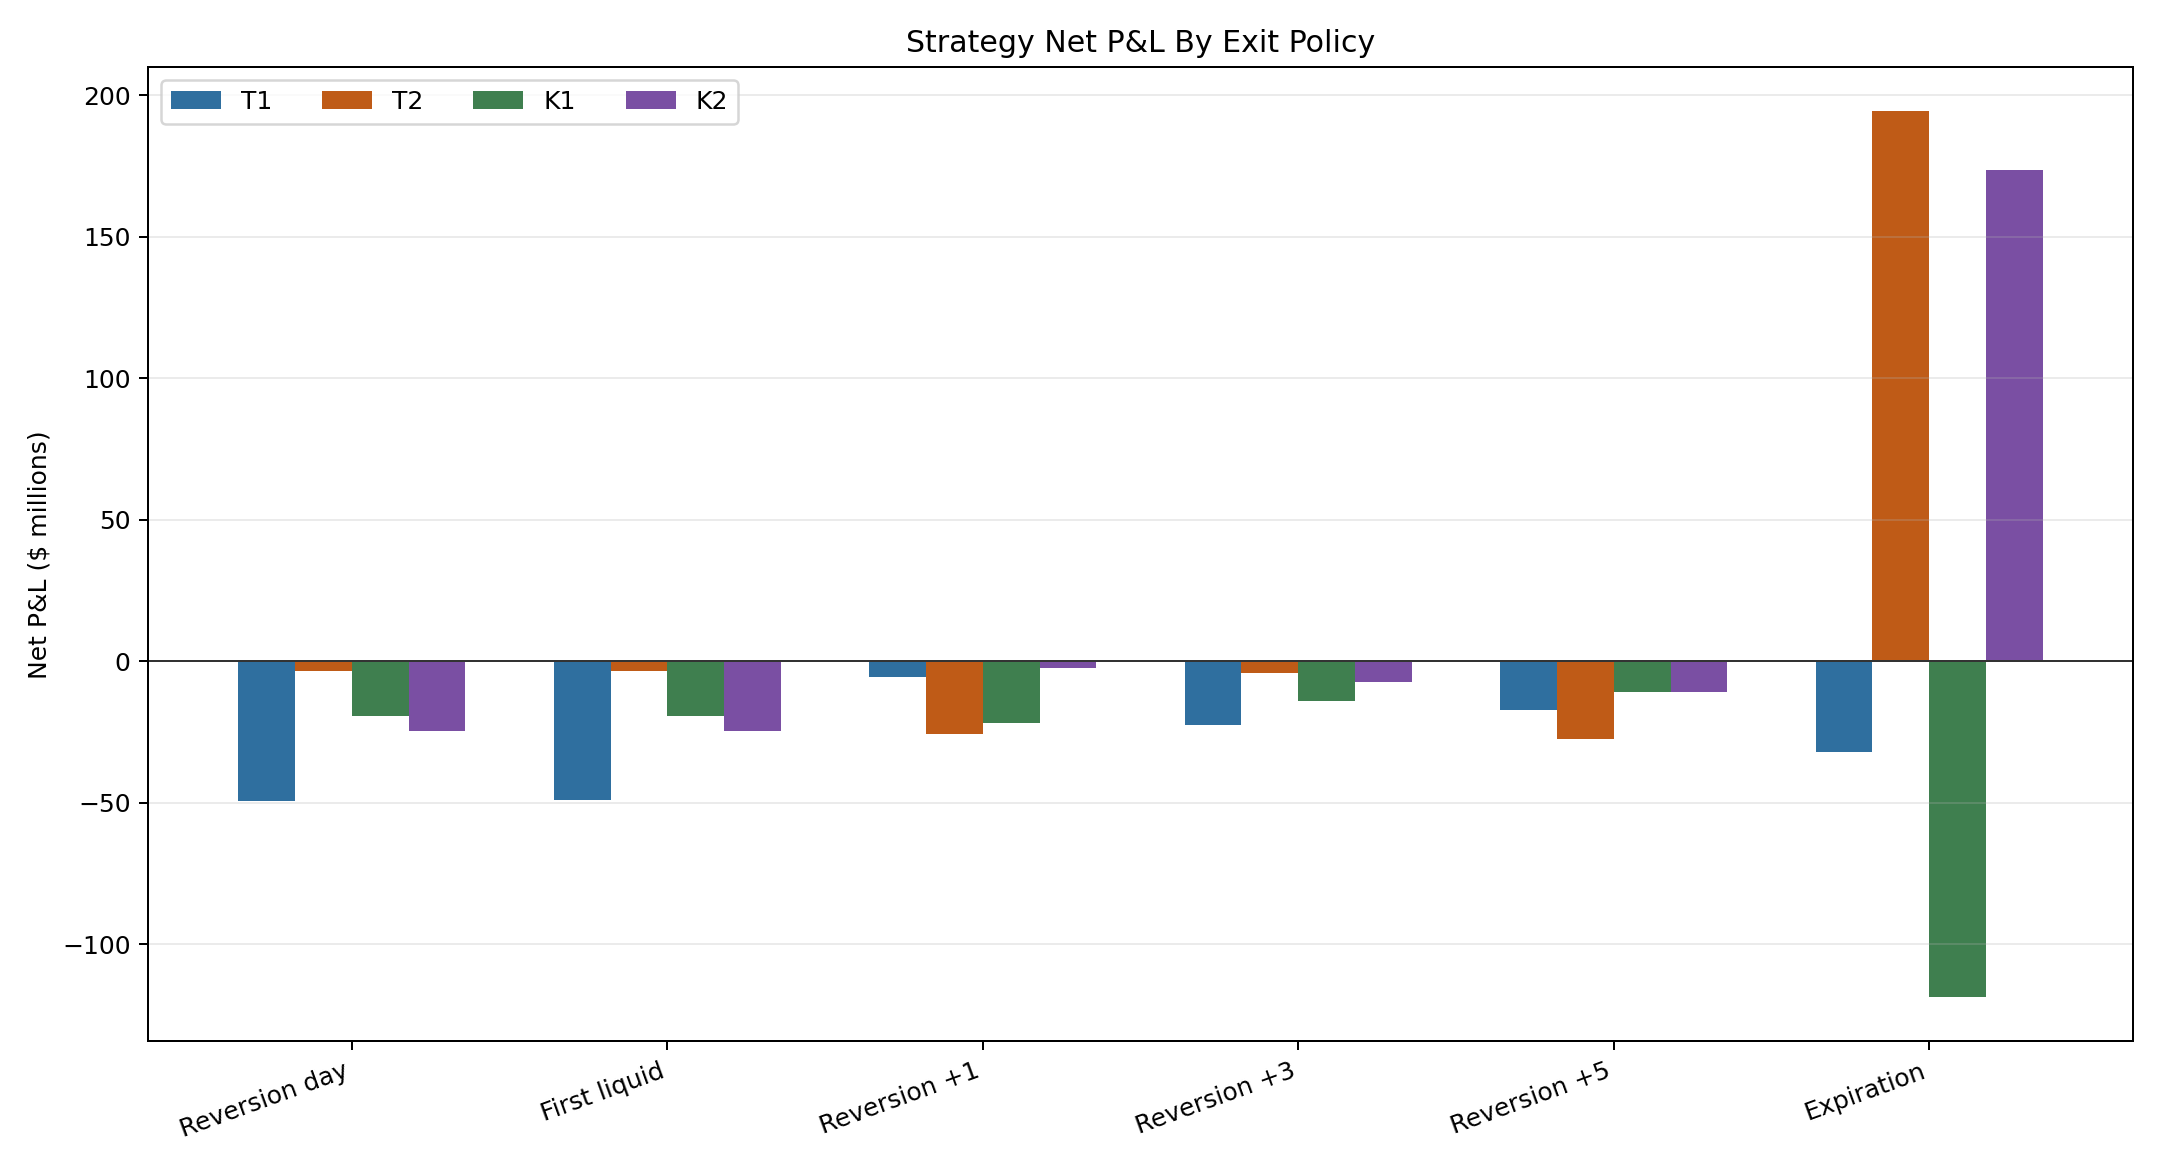
\includegraphics[width=0.92\linewidth]{figures/strategy_robustness_policy_pnl.png}
  \caption{Strategy net P\&L by exit policy.}
\end{figure}

\begin{figure}[H]
  \centering
  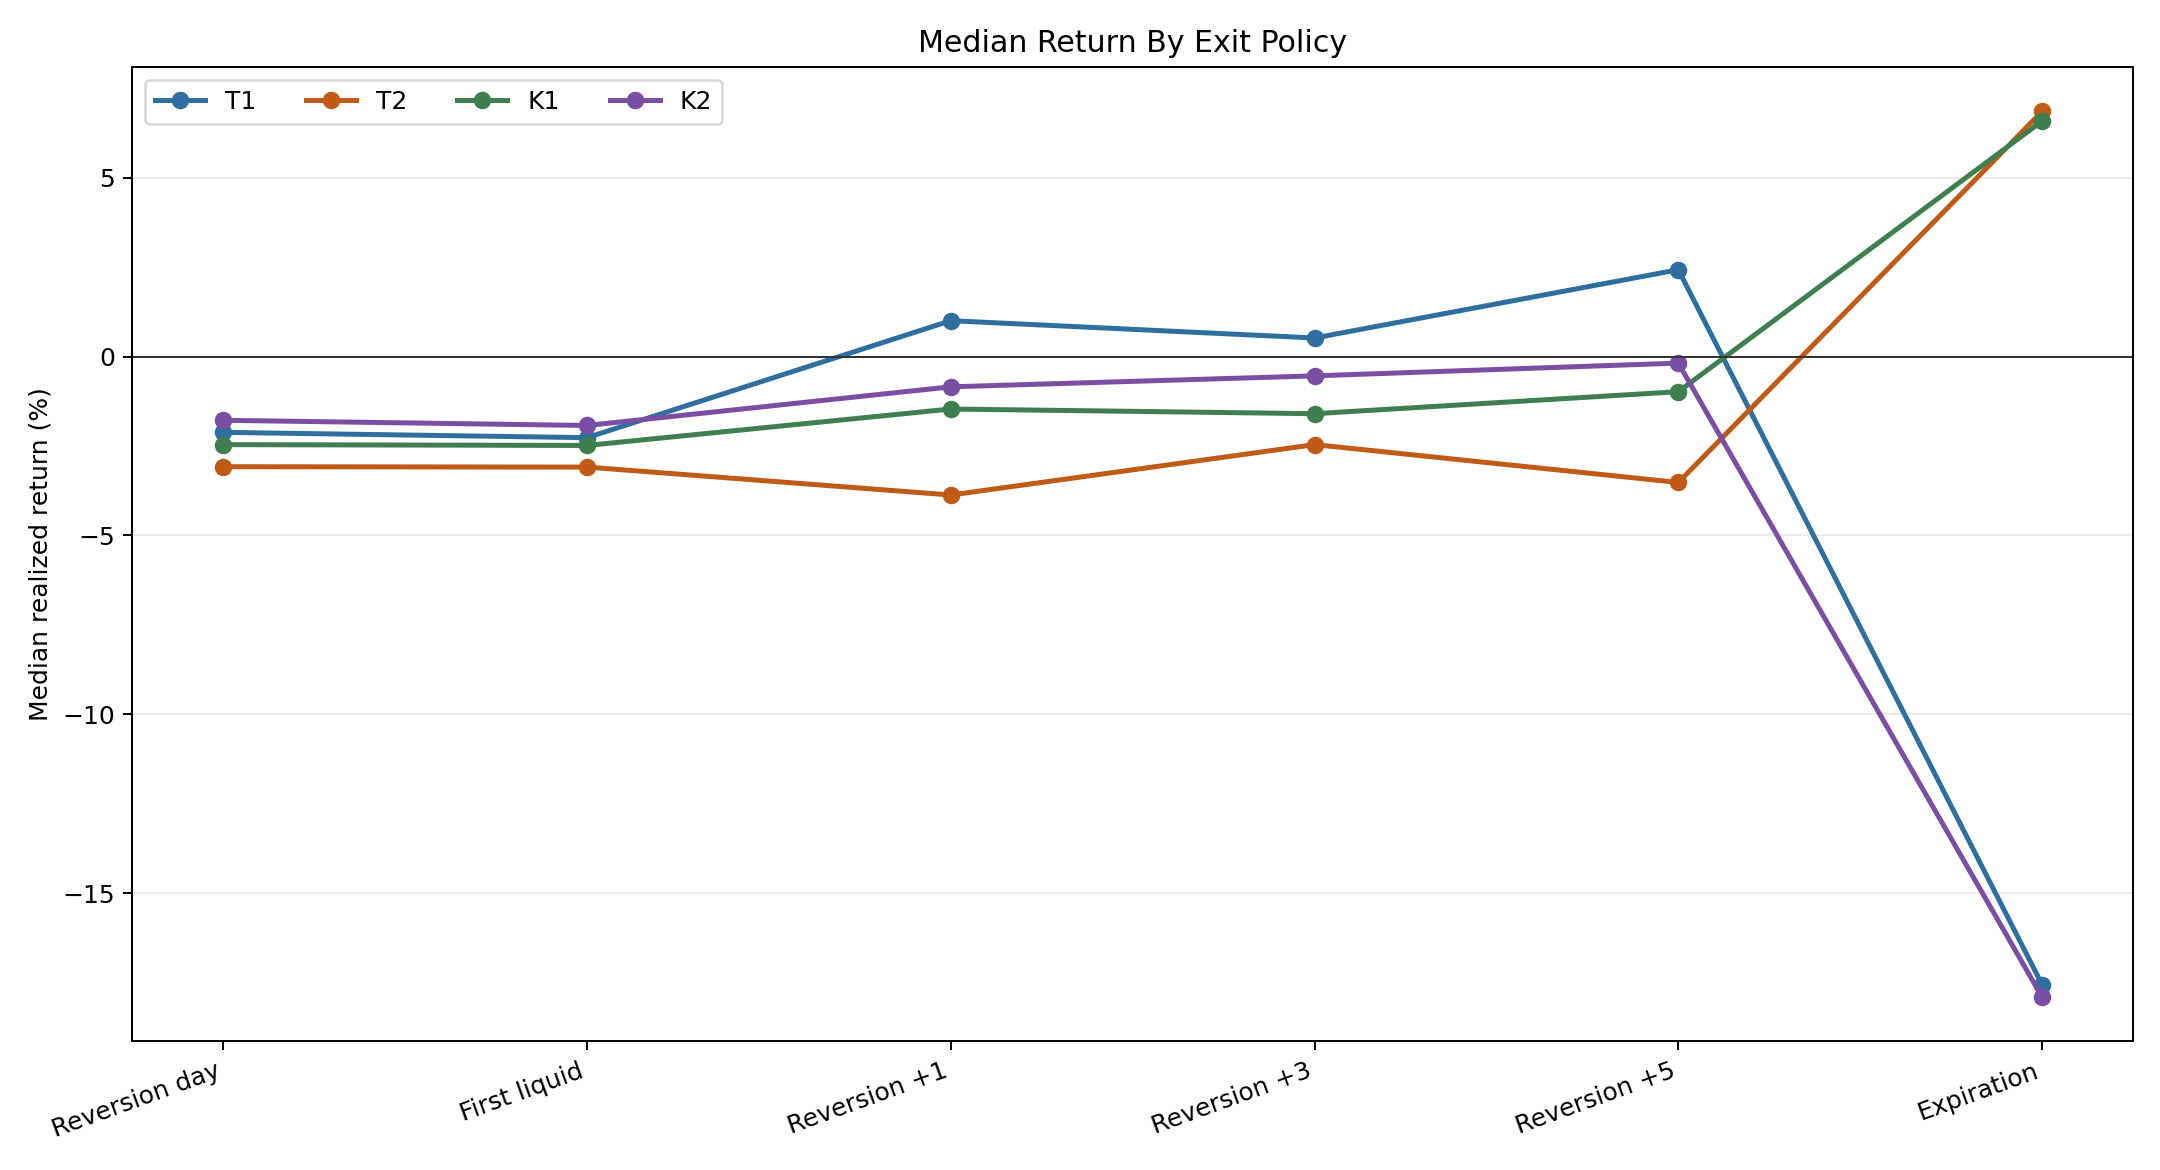
\includegraphics[width=0.92\linewidth]{figures/strategy_robustness_median_return.png}
  \caption{Median realized return by exit policy.}
\end{figure}

\begin{figure}[H]
  \centering
  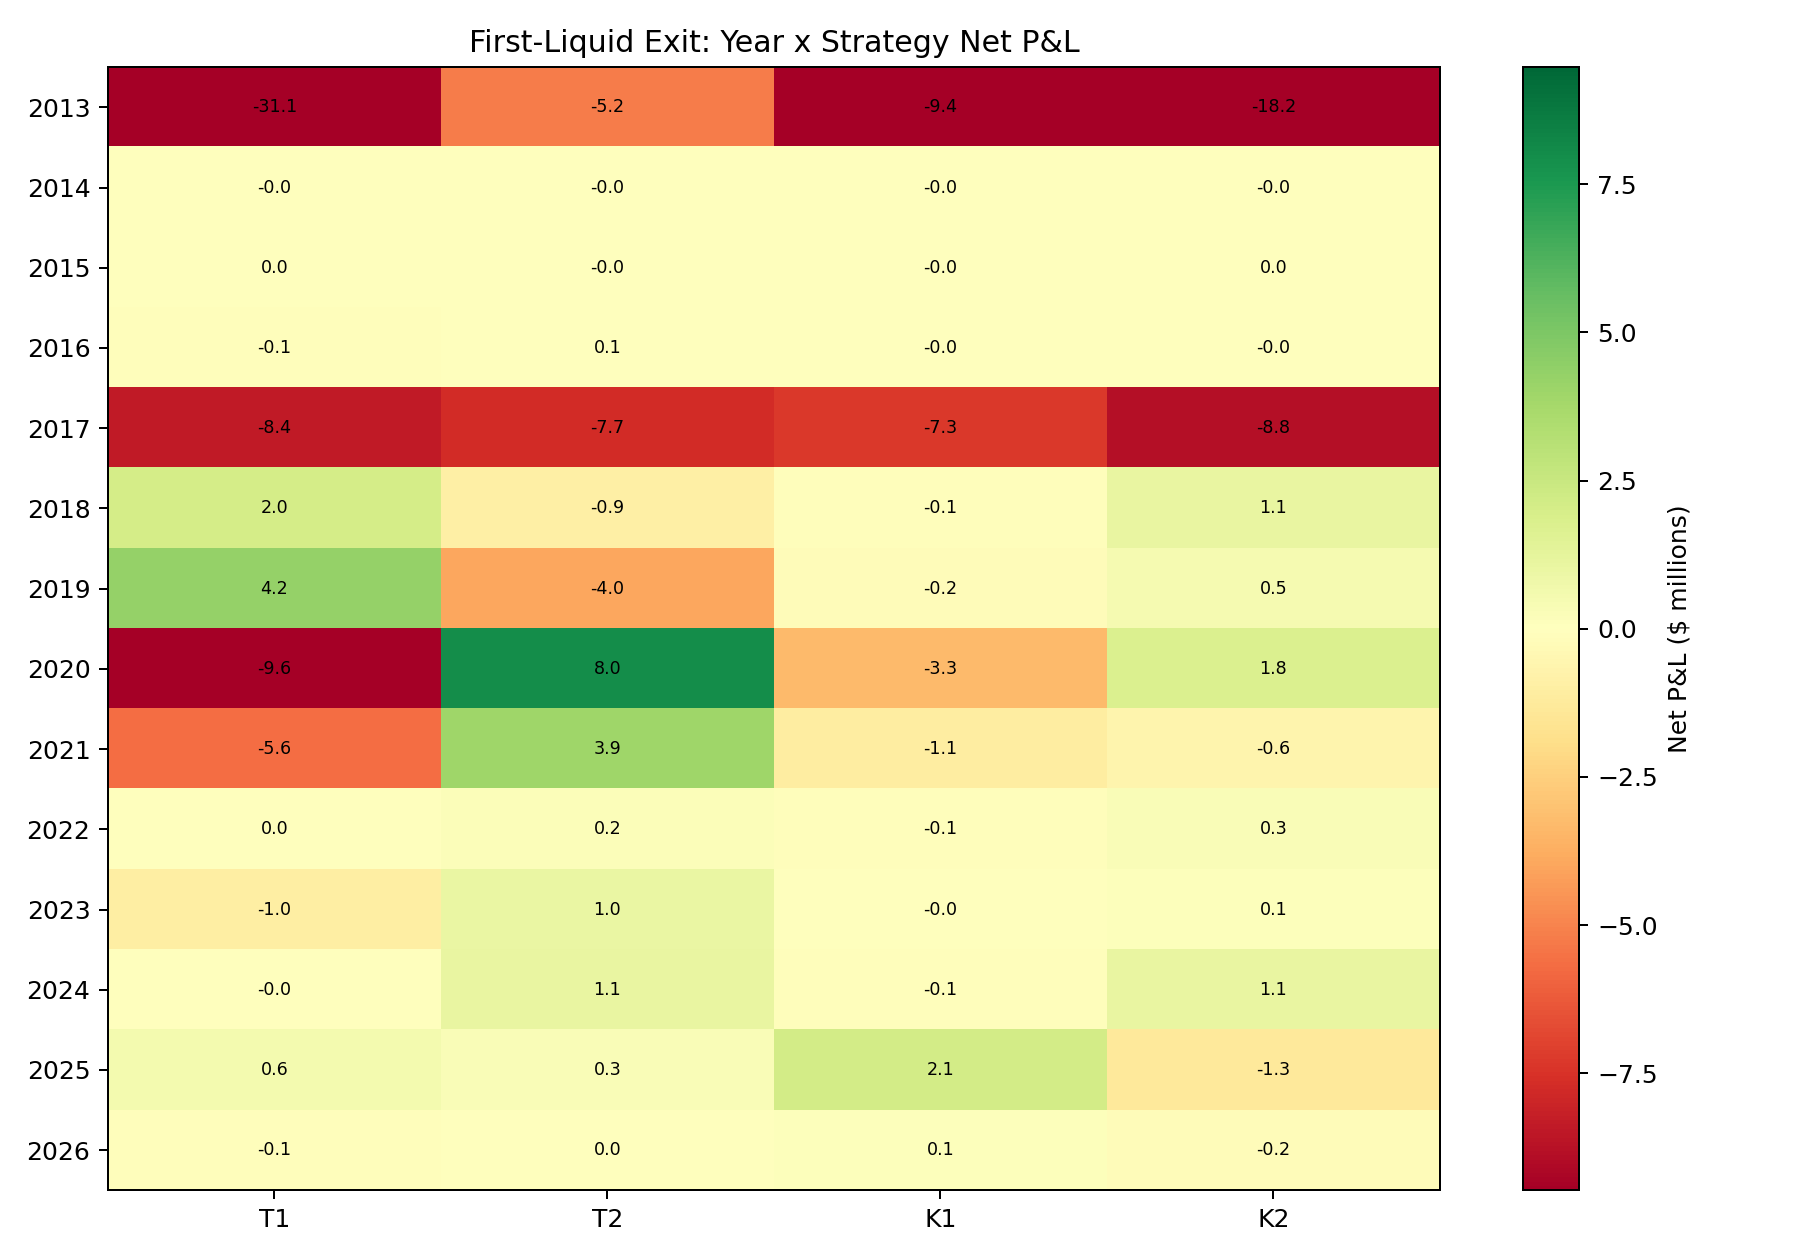
\includegraphics[width=0.92\linewidth]{figures/strategy_robustness_first_liquid_year_heatmap.png}
  \caption{First-liquid exit year-by-strategy net P\&L heatmap.}
\end{figure}


\section{Interpretation}

Only two of the twenty-four policy-strategy cells are positive in aggregate.
Unconditional premium-resale trading is fragile. Expiration payoff behaves
differently from first-liquid premium resale, so the paper should report those
as separate benchmarks. The defensible claim is ML-based selection of tradeable
TP2 episodes, not universal arbitrage from every violation.

\end{document}
